\begin{savequote}[45mm]
\ascii{Any fool can write code that a computer can understand. Good programmers write code that humans can understand.}
\qauthor{\ascii{- Martin Flower}}
\end{savequote}

\chapter{BP算法} 
\label{ch:bp}

\begin{content}

\end{content}

\section{TensorFlow实现}

\begin{content}

\tf{}是一个实现了自动微分的软件系统。首先,它构造正向的计算图,实现计算图的前向计算。当调用\code{Optimizer.minimize}方法时,使用\code{compute\_gradients}方法,实现反向计算图的构造;使用\code{apply\_gradients}方法,实现参数更新的子图构造。

\begin{leftbar}
\begin{python}
class Optimizer(object):
  def minimize(self, loss, var_list=None, global_step=None):
    """Add operations to minimize loss by updating var_list.
    """
    grads_and_vars = self.compute_gradients(
      loss, var_list=var_list)
    return self.apply_gradients(
      grads_and_vars, 
      global_step=global_step)
\end{python}
\end{leftbar}

\subsection{计算梯度}

\code{compute\_gradients}将根据\code{loss}的值,求解\code{var\_list=[v1, v2, ..., vn]}的梯度,最终返回的结果为:\code{[(grad\_v1, v1), (grad\_v2, v2), ..., (grad\_vn, vn)]}。其中,\code{compute\_gradients}将调用\code{gradients}方法,构造反向传播的子图。

以一个简单实例,讲解反向子图的构造过程。首先,构造前向的计算图。

\begin{leftbar}
\begin{python}
X = tf.placeholder("float", name="X")
Y = tf.placeholder("float", name="Y")
w = tf.Variable(0.0, name="w")
b = tf.Variable(0.0, name="b")
loss = tf.square(Y - X*w - b)
global_step = tf.Variable(0, trainable=False, collections=[])
\end{python}
\end{leftbar}

使用\code{compute\_gradients}构造反向传播的子图。

\begin{leftbar}
\begin{python}
sgd = tf.train.GradientDescentOptimizer(0.01)
grads_and_vars = sgd.compute_gradients(loss)
\end{python}
\end{leftbar}

\subsubsection{构造算法}

反向子图的构建算法可以形式化地描述为:

\begin{leftbar}
\begin{python}
def gradients(loss, grad=I):
  vrg = build_virtual_reversed_graph(loss)
  for op in vrg.topological_sort():
    grad_fn = ops.get_gradient_function(op)
    grad = grad_fn(op, grad)
\end{python}
\end{leftbar}

首先,根据正向子图的拓扑图,构造一个虚拟的反向子图。之所以称为虚拟的,是因为真实的反向子图要比它复杂得多;更准确的说,虚拟的反向子图中的一个节点,对应于真实的反向子图中的一个局部子图。

同时,正向子图输出的最后一个节点,其输出梯度全为\ascii{1}的一个\code{Tensor},作为反向子图的初始的梯度值,常常记为\code{I}。

\begin{figure}[!htbp]
\centering
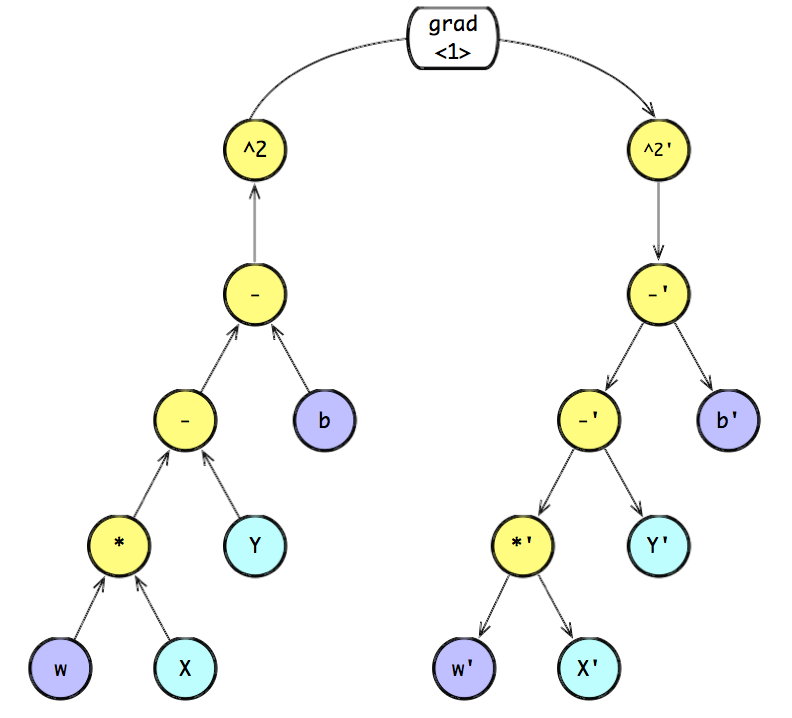
\includegraphics[width=0.7\textwidth]{figures/bp-back-graph-construction.png}
\caption{构造反向传播子图}
 \label{fig:bp-back-graph-construction}
\end{figure}

接下来,根据虚拟的反向子图构造真实的反向子图。首先,根据该反向的虚拟子图执行拓扑排序算法,得到该虚拟的反向子图的一个拓扑排序;然后,按照该拓扑排序,对每个正向子图中的\ascii{OP}寻找其「梯度函数」;最后,调用该梯度函数,该梯度函数将构造该\ascii{OP}对应的反向的局部子图。

综上述,正向的一个\ascii{OP}对应反向的一个局部子图,并由该\ascii{OP}的梯度函数负责构造。当整个拓扑排序算法完成后,正向子图中的每个\ascii{OP}在反向子图中都能找到对应的局部子图。

例如,在上例中,正向图中最后一个\ascii{OP}:求取平方的函数为例,讲述梯度函数的工作原理。

\subsubsection{梯度函数原型}

一般地,梯度函数满足如下原型:

\begin{leftbar}
\begin{python}
@ops.RegisterGradient("op_name")
def op_grad_func(op, grad):
\end{python}
\end{leftbar}

其中,梯度函数由\code{ops.RegisterGradient}完成注册,并放在保存梯度函数的仓库中。以后,便可以根据正向\ascii{OP}的名字,索引对应的梯度函数了。

对于一个梯度函数,第一个参数\code{op}表示正向计算的\ascii{OP},根据它可以获取正向计算时\ascii{OP}的输入和输出;第二个参数\code{grad},是反向子图中上游节点传递过来的梯度,它是一个已经计算好的梯度值(初始梯度值全为1)。

\subsubsection{实战:平方函数}

举个简单的例子,仅使用输入计算梯度。\code{y=square(x)},用于求取\code{x}的平方。首先,构造正向计算图:

\begin{figure}[!h]
\centering
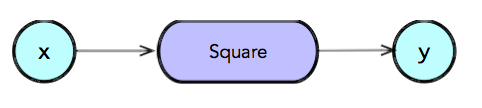
\includegraphics[width=0.5\textwidth]{figures/bp-square-forward-graph.png}
\caption{Square函数:正向传播子图}
 \label{fig:bp-square-forward-graph}
\end{figure}

然后,反向构造虚拟的反向子图。根据该虚拟的反向子图的拓扑排序,构造真正的反向计算子图。假如,当前节点为\code{Square},根据其OP名称,从仓库中找到对应的梯度函数\code{SquareGrad}。

\begin{figure}[!htbp]
\centering
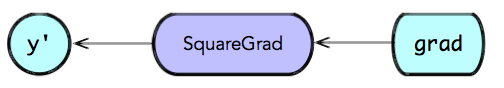
\includegraphics[width=0.5\textwidth]{figures/bp-square-backward-graph.png}
\caption{Square函数:反向传播子图}
 \label{fig:bp-square-backward-graph}
\end{figure}

因为,\code{y=Square(x)}的导数为\code{y'=2*x}。因此,其梯度函数\code{SquareGrad}的实现为:

\begin{leftbar}
\begin{python}
@ops.RegisterGradient("Square")
def SquareGrad(op, grad):
  x = op.inputs[0]
  with ops.control_dependencies([grad.op]):
    x = math_ops.conj(x)
    return grad * (2.0 * x)
\end{python}
\end{leftbar}

调用该梯度函数后,将得到正向\code{Square}的\ascii{OP},对应的反向子图\code{SquareGrad}。它需要使用\code{Square}的输入,完成相应的梯度计算。

\begin{figure}[!h]
\centering
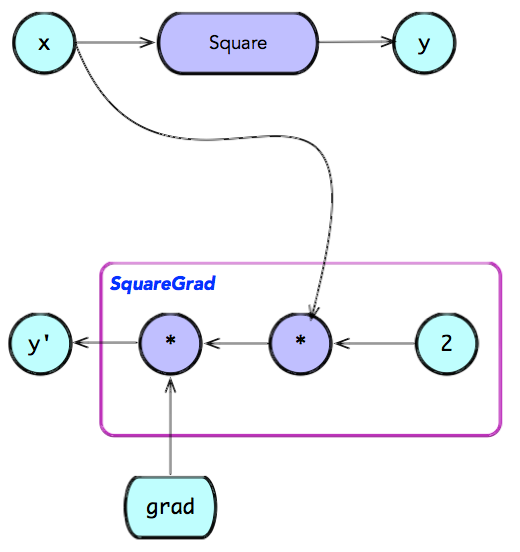
\includegraphics[width=0.5\textwidth]{figures/bp-square-backward-graph-2.png}
\caption{Square函数:反向传播子图}
 \label{fig:bp-square-backward-graph-2}
\end{figure}

一般地,正向子图中的一个\ascii{OP},对应反向子图中的一个局部子图。因为,正向\ascii{OP}的梯度函数实现,可能需要多个\ascii{OP}才能完成相应的梯度计算。例如,\code{Square}的\ascii{OP},对应梯度函数构造了包含两个\ascii{2}个乘法\ascii{OP}。

\subsubsection{实战:指数函数}

再举个简单的例子,仅使用输出计算梯度。\code{y=exp(x)},指数函数;其导数为\code{y'=exp(x)},即\code{y'=y}。因此,其梯度函数实现为:

\begin{leftbar}
\begin{python}
@ops.RegisterGradient("Exp")
def _ExpGrad(op, grad):
  """Returns grad * exp(x)."""
  y = op.outputs[0]
  with ops.control_dependencies([grad.op]):
    y = math_ops.conj(y)
    return grad * y
\end{python}
\end{leftbar}

如下图所示,正向子图中该\ascii{OP}的输出,用于对应的反向的局部子图的梯度运算。而且,该局部子图进包含一个节点。

\begin{figure}[!h]
\centering
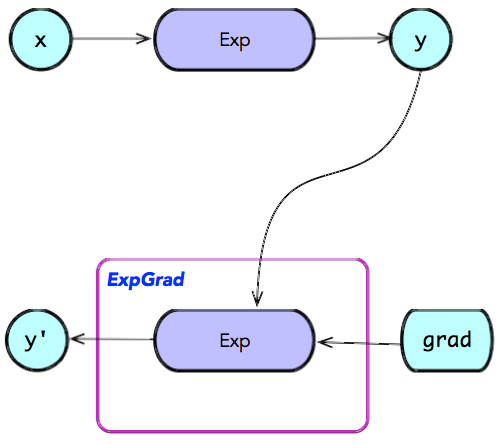
\includegraphics[width=0.5\textwidth]{figures/bp-exp-backward-graph.png}
\caption{Exp函数:反向传播子图}
 \label{fig:bp-exp-backward-graph}
\end{figure}

\subsection{应用梯度}

再做一个简单的总结,当调用\code{Optimizer.minimize}方法时,使用\code{compute\_gradients}方法,实现反向计算图的构造;使用\code{apply\_gradients}方法,实现参数更新的子图构造。

\subsubsection{构造算法}

首先,\code{compute\_gradients}在运行时将根据\code{loss}的值,求解\code{var\_list=[v1, v2, ..., vn]}的梯度,最终返回的结果为:\code{vars\_and\_grads = [(grad\_v1, v1), (grad\_v2, v2), ..., (grad\_vn, vn)]}。

然后,\code{apply\_gradients}迭代\code{grads\_and\_vars},对于每个\code{(grad\_vi, vi)},构造一个更新\code{vi}的子图。其中,算法可以形式化地描述为:

\begin{leftbar}
\begin{python}
def apply_gradients(grads_and_vars, learning_rate):
  for (grad, var) in grads_and_vars:
    apply_gradient_descent(learning_rate, grad, var)
\end{python}
\end{leftbar}

其中,\code{apply\_gradient\_descent}将构造一个使用梯度下降算法更新参数的计算子图。将\code{(grad, var)}的二元组,及其\code{learning\_rate}的\code{Const OP}作为\code{ApplyGradientDescent}的输入。

\code{ApplyGradientDescent}将应用\code{var <- var - learning*grad}的运算规则,实现\code{var}的就地更新。

\begin{figure}[!h]
\centering
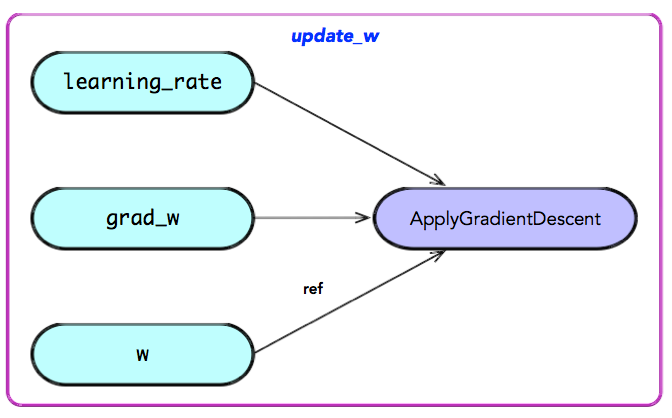
\includegraphics[width=0.6\textwidth]{figures/bp-update-w.png}
\caption{参数更新子图}
 \label{fig:bp-update-w}
\end{figure}

\subsubsection{参数更新汇总}

如果存在多个训练的Variable,最终生成多个更新参数的局部子图。它们通过一个名为\code{update}的\code{NoOp},使用控制依赖边汇总在一起。因为各个\code{Variable}之间相互独立,可以实现最大化的并发。

\begin{figure}[!h]
\centering
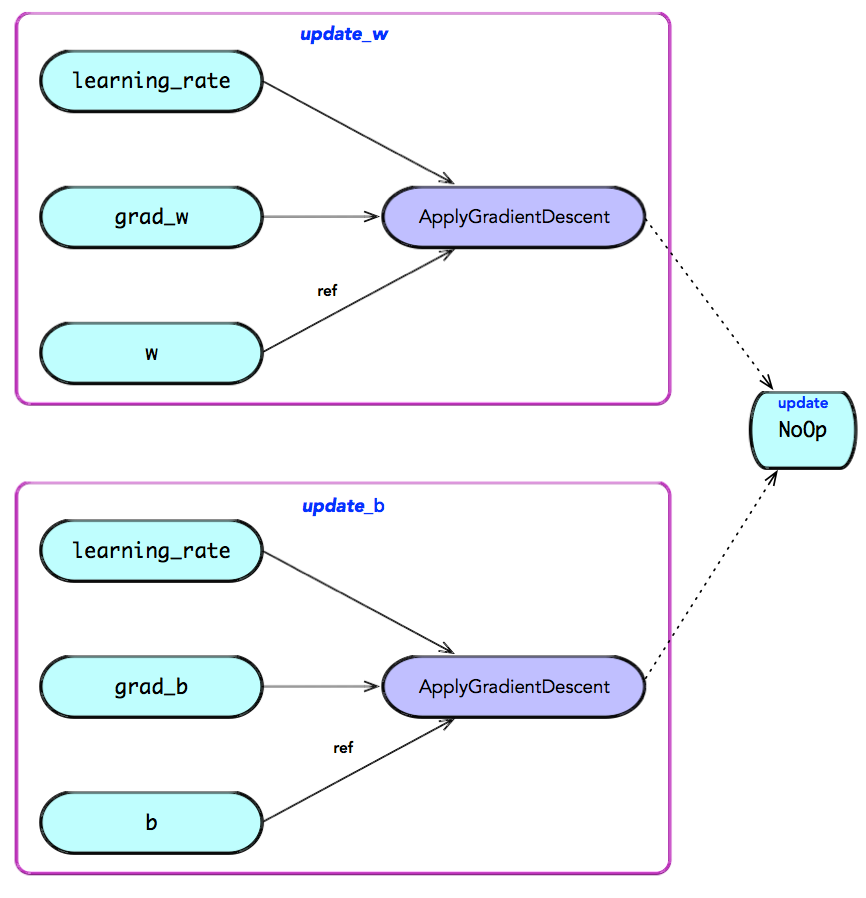
\includegraphics[width=0.9\textwidth]{figures/bp-update-all-params.png}
\caption{参数更新汇总}
 \label{fig:bp-update-all-params}
\end{figure}

\subsubsection{探秘train\_op}

经过一轮\ascii{Step}运算,根据梯度,完成参数的更新,最终完成\code{global\_step}加1。而实现\code{global\_step}加\ascii{1}的\ascii{OP}为\code{AssignAdd},并标记为\code{train\_op};它持有\code{global\_step}变量的引用,然后完成就地修改,使其值加\ascii{1}。

\begin{figure}[!h]
\centering
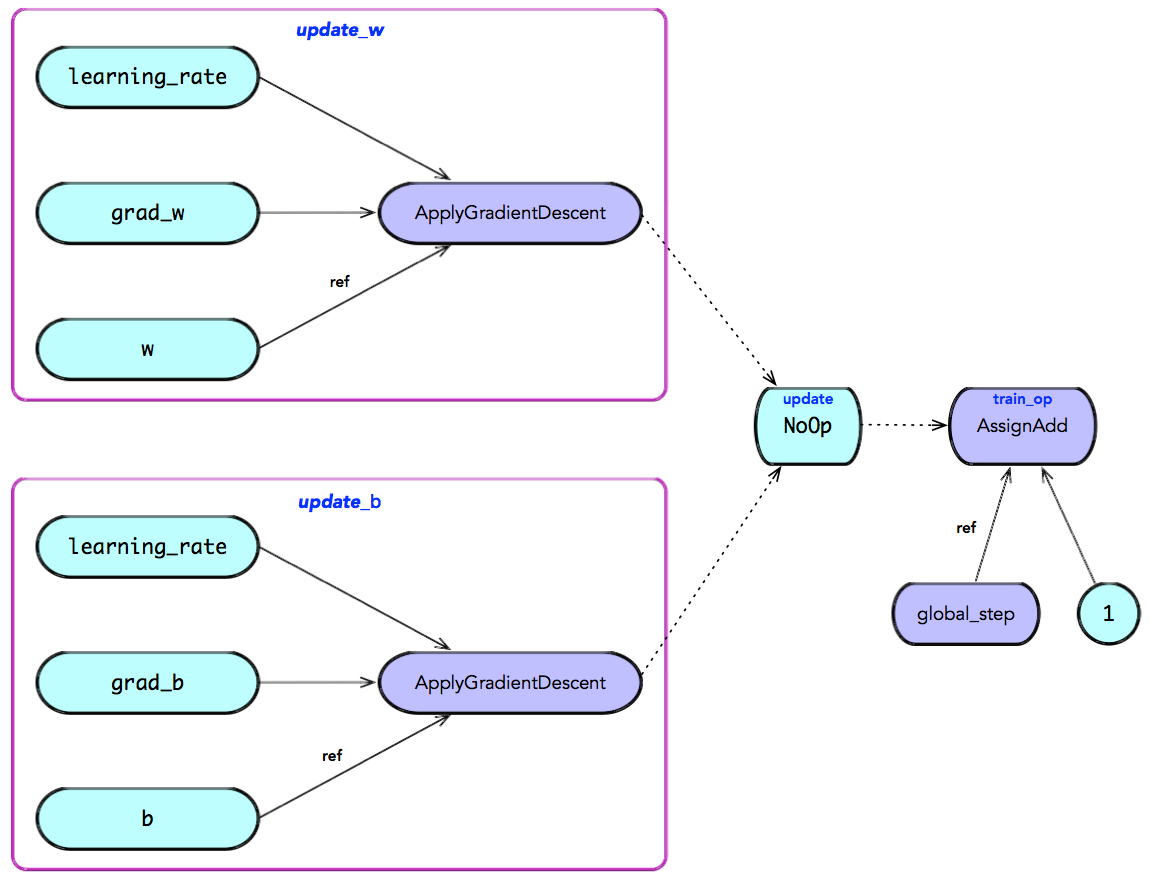
\includegraphics[width=0.9\textwidth]{figures/bp-train-op.png}
\caption{train\_op}
 \label{fig:bp-train-op}
\end{figure}

\subsubsection{工作流}

如\refig{bp-train-pipeline}所示,整个训练过程,一次\ascii{Step}的训练过程由前向计算,反向梯度计算,参数更新,及其\code{global\_step}计数四个基本过程组成。

其中,每一轮\ascii{Step}从开始\code{Session.run}执行开始。通过前向子图的计算,得到每个\ascii{OP}的输出,并作为下游\ascii{OP}的输入。

当前向子图完成计算后,再以初始梯度向量$ I $为输入,反向计算各个训练参数的梯度,最终得到各个训练参数的梯度列表,并以\code{grads\_and\_vars = [(grad\_v1, v1), ..., (grad\_vn, vn)]}的二元组列表表示。

随后,参数更新子图以\code{grads\_and\_vars}为输入,执行梯度下降的更新算法;最后,通过\code{train\_op}完成\code{global\_step}值加\ascii{1},至此一轮\ascii{Step}执行完成。

\begin{figure}[!h]
\centering
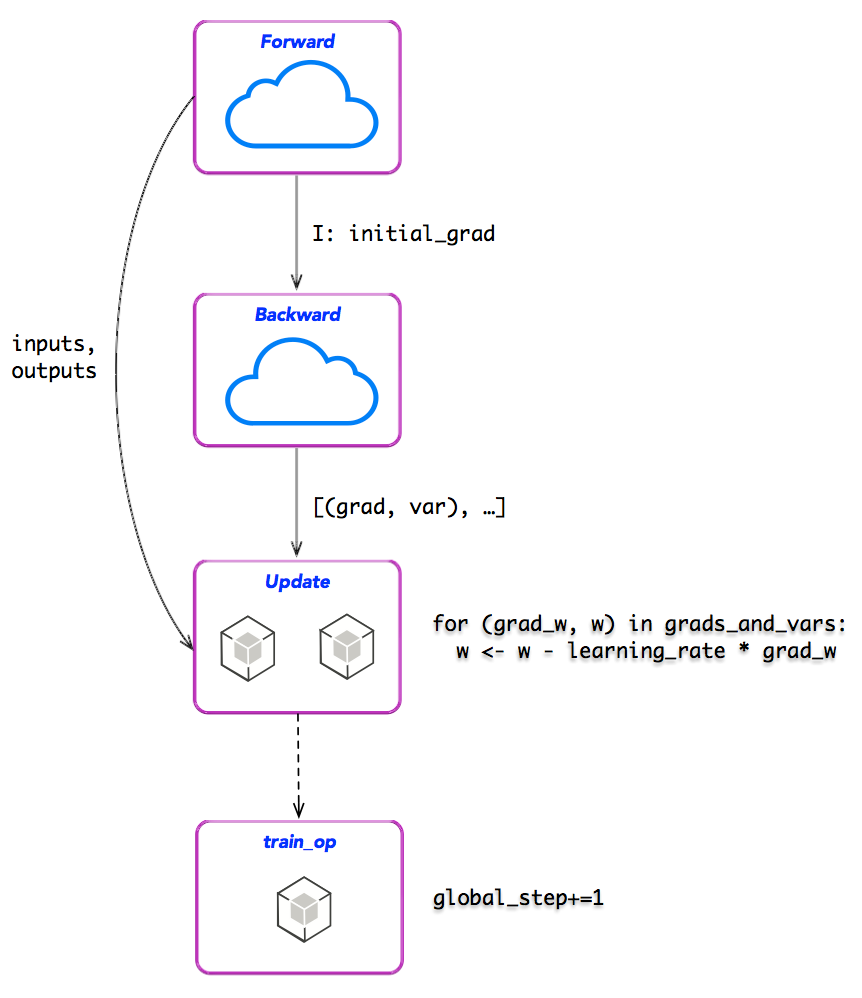
\includegraphics[width=0.9\textwidth]{figures/bp-train-pipeline.png}
\caption{模型训练的工作流}
 \label{fig:bp-train-pipeline}
\end{figure}

\end{content}
